\section{Tables SQL Radius}

\subsection{RadCheck}

La table \textit{radcheck} permet de stocker les différentes conditions que doit remplir un utilisateur pour obtenir une autorisation de connexion. La structure de la table est la suivante :

\begin{verbatim}
+----+----------+-----------+----+-------+
| id | username | attribute | op | value |
+----+----------+-----------+----+-------+
\end{verbatim}

Chaque enregistrement correspond à une condition. On précise l'utilisateur concerné (username), le nom de l'attribut à vérifier (attribute), un opérateur (op) et la valeur de référence (value). Ils existent plusieurs types d'opérateurs :

\begin{tabular}{|r|l|}
	\hline
  \textbf{Opérateur} & \textbf{Action} \\
  \hline
  = & Uniquement pour les paramètres serveur (Auth-Type...). \\
	  & Il modifie la valeur configurée sur le serveur si aucun autre paramètre ne l'a fait. \\
  \hline
  := & Remplace n'importe quel attribut dans la liste des éléments de configuration et le crée s'il n'existe pas. \\
  \hline
  == & Vérifie que l'attribut est présent dans la réponse et s'il a la bonne valeur. \\
  \hline
  += & Ajoute l'attribut avec sa valeur à la liste des éléments de configuration. \\
  \hline
  != & Vérifie que l'attribut est présent dans la réponse et s'il n'a pas la valeur spécifiée. \\
  \hline
  > & Vérifie que l'attribut est présent dans la réponse et si sa valeur est supérieure à celle spécifiée. \\
  \hline
  >= & Vérifie que l'attribut est présent dans la réponse et si sa valeur est supérieure ou égale à celle spécifiée. \\
  \hline
  < & Vérifie que l'attribut est présent dans la réponse et si sa valeur est inférieure à celle spécifiée. \\
  \hline
  <= & Vérifie que l'attribut est présent dans la réponse et si sa valeur est inférieure ou égale à celle spécifiée. \\
  \hline
  =~ & Vérifie que l'attribut est présent dans la réponse et si sa valeur correspond à l'expression régulière. \\
		 & Uniquement pour les attributs dont le type est chaîne de caractère. \\
  \hline
  !~ & Vérifie que l'attribut est présent dans la réponse et si sa valeur ne correspond pas à l'expression régulière. \\
		 & Uniquement pour les attributs dont le type est chaîne de caractère. \\
  \hline
  =* & Vérifie que l'attribut est présent dans la réponse, peu importe sa valeur. \\
  \hline
  !* & Vérifie que l'attribut n'est pas présent dans la réponse. \\
	\hline
\end{tabular}

La reqête SQL pour ajouter une condition est :

\begin{verbatim}
INSERT INTO radcheck (username, attribute, op, value)
            VALUES ('user1', 'attributeName', ':=', 'valueString');
\end{verbatim}

Ci-dessous sont listés différentes conditions qui peuvent nous intéresser :

\begin{tabular}{rl}
  \multicolumn{2}{l}{Mot de passe} \\
  \hline
  Attribute & Cleartext-Password \\
  Requête & ('user1', 'Cleartext-Password', 'pass1'); \\
  \\
  \multicolumn{2}{l}{Mot de passe chiffré} \\
  \hline
  Attribute & Crypt-Password \\
  Requête & ('user1', 'Crypt-Password', encrypt('pass1')); \\
  \\
  \multicolumn{2}{l}{Mot de passe MD5} \\
  \hline
  Attribute & MD5-Password \\
  Requête & ('user1', 'MD5-Password', MD5('pass1')); \\
  \\
	\multicolumn{2}{l}{Date d'expiration du compte} \\
  \hline
  Attribute & Expiration \\
  Requête & ('user1', 'Expiration', '17 oct 2012 19:00:00'); \\
	Remarque & Le format de la date est "\textit{dd m YYYY HH:ii:ss}" (à vérifier) \\
	\\
	\multicolumn{2}{l}{Horraires d'accès} \\
  \hline
  Attribute & Login-Time \\
  Requête & ('user1', 'Login-Time', 'any0700-2000'); \\
	Remarque & Le format est une composition de contrainte séparée par des ',' ou des '|'. \\
					 & On précise jour et heure. \\
					 & Du lundi au vendredi : Wk \\
					 & Un jour particulier : Mo,Tu,We,Th,Fr,Sa,Su \\
					 & Tout : Any ou All \\
					 & Horaires : 0800-2000 (entre 8h et 20h) \\
					 & Jamais: Never \\
	\\
	\multicolumn{2}{l}{Nombre de connexion simultanéee (non testé)} \\
  \hline
  Attribute &  Simultaneous-Use \\
  Requête & ('user1', ' Simultaneous-Use', '2'); \\
	Remarque & Il est nécessaire d'activer l'accounting pour que cette option fonctionne.
	\\
	\multicolumn{2}{l}{Type d'authentification (non testé)} \\
  \hline
  Attribute &  Auth-Type \\
  Requête & ('user1', ' Auth-Type', 'EAP'); \\
	Remarque & Les valeurs possibles sont : EAP, ... (à compléter) \\
	\\
	\multicolumn{2}{l}{Type d'authentification} \\
  \hline
  Attribute &  EAP-Type \\
  Requête & ('user1', ' EAP-Type', 'MD5-CHALLENGE'); \\
	remarque & Les valeurs possibles sont : MD5-CHALLENGE, EAP-TLS, EAP-TTLS, PEAP... (à compléter) \\
	\\
	\multicolumn{2}{l}{Type de connexion (Dot1X, Console, VTY..)} \\
  \hline
  Attribute &  NAS-Port-Type \\
  Requête & ('user1', ' NAS-Port-Type', '==', '15'); \\
	Remarque & Les valeurs possibles sont : 15 (Ethernet/Dot1x), 0 Console, 5 VTY, ... (à compléter) \\
	\\
	\multicolumn{2}{l}{IP du NAS (non testé)} \\
  \hline
  Attribute &  NAS-IP-Address \\
  Requête & ('user1', ' NAS-IP-Address', '==', '192.168.0.254'); \\
	\\
	\multicolumn{2}{l}{MAC du NAS (non testé)} \\
  \hline
  Attribute &  Called-Station-Id \\
  Requête & ('user1', ' Called-Station-Id', '==', '0123456789ab'); \\
	\\
	\multicolumn{2}{l}{MAC de l'utilisateur (non testé)} \\
  \hline
  Attribute &  Calling-Station-Id \\
  Requête & ('user1', ' Calling-Station-Id', '==', '06656343bjdfbg'); \\
	\\
\end{tabular}

Ci-dessous, la liste des compatibilité entre les types de mots de passe stockés dans la base de donnée et les méthodes d'authentification :

\begin{center}
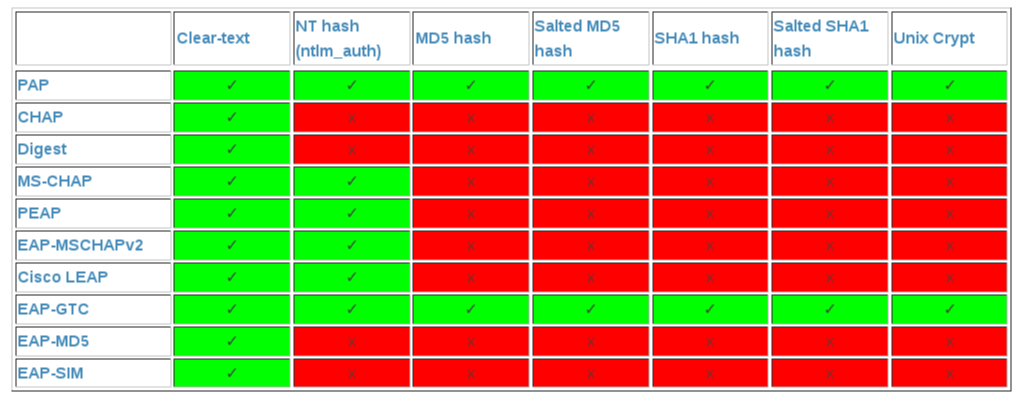
\includegraphics[width=400pt]{img/password_compatibility.png}
\end{center}

\subsection{RadGroupCheck}

La table \textit{radgroupcheck} permet de stocker les différentes conditions que doit remplir un groupe pour obtenir une autorisation de connexion. La structure de la table est la suivante :

\begin{verbatim}
+----+----------+-----------+----+-------+
| id | xxxxxxxx | attribute | op | value |
+----+----------+-----------+----+-------+
\end{verbatim}

Son fonctionnement est le même que la table \textit{radcheck}.

\subsection{RadReply}

La table \textit{radreply} recense les informations à renvoyer à l'utilisateur authentifié. Par exemple, le VLAN auquel il sera connecté. La structure de la table est la suivante :

\begin{verbatim}
+----+----------+-----------+----+-------+
| id | username | attribute | op | value |
+----+----------+-----------+----+-------+
\end{verbatim}

Chaque enregistrement correspond à un attribut de la réponse. On précise l'utilisateur concerné (username), le nom de l'attribut à vérifier (attribute), un opérateur (op) et la valeur (value). Ils existent plusieurs types d'opérateurs :

\begin{tabular}{|r|l|}
	\hline
  \textbf{Opérateur} & \textbf{Action} \\
  \hline
  = & Ajout l'attribut à la réponse uniquement s'il n'existe pas déjà. \\
  \hline
  := & Remplace n'importe quel attribut dans la liste des attributs de réponse et le crée s'il n'existe pas. \\
  \hline
  == & Non autorisé. \\
  \hline
  += & Ajoute l'attribut avec sa valeur à la réponse. \\
  \hline
  != & Non autorisé. \\
  \hline
  > & Non autorisé. \\
  \hline
  >= & Non autorisé. \\
  \hline
  < & Non autorisé. \\
  \hline
  <= & Non autorisé. \\
  \hline
  =~ & Non autorisé. \\
  \hline
  !~ & Non autorisé. \\
  \hline
  =* & Non autorisé. \\
  \hline
  !* & Non autorisé. \\
	\hline
\end{tabular}

La reqête SQL pour ajouter un attribut de réponse est :

\begin{verbatim}
INSERT INTO radreply (username, attribute, op, value)
            VALUES ('user1', 'attributeName', '=', 'valueString');
\end{verbatim}

Ci-dessous sont listés différentes conditions qui peuvent nous intéresser :

\begin{tabular}{rl}
  \multicolumn{2}{l}{Affectation VLAN} \\
  \hline
  Attribute & Tunnel-Type \\
  Valeur & "VLAN" \\
	Requête & ('user1', 'Tunnel-Type', '=', 'VLAN'); \\
  \\
  Attribute & Tunnel-Medium-Type \\
  Valeur & "IEEE-802" \\
	Requête & ('user1', 'Tunnel-Medium-Type', '=', 'IEEE-802'); \\
  \\
  Attribute & Tunnel-Private-Group-Id \\
  Valeur & Numéro du VLAN \\
	Requête & ('user1', 'Tunnel-Private-Group-Id', '=', '42'); \\
  \\
	\multicolumn{2}{l}{Message} \\
  \hline
  Attribute & Reply-Message \\
  Valeur & Un message qui sera affiché chez l'utilisateur \\
	Requête & ('user1', 'Reply-Message', '=', 'Bonjour {\%User-Name}'); \\
	\\
	\multicolumn{2}{l}{Exécuter un programme et attendre son exécution (non testé)} \\
  \hline
  Attribute &  Exec-Program-Wait \\
  Requête & ('user1', 'Exec-Program-Wait', '=', '/usr/local/bin/un-programme 3 dupont “30 Mar 2007 00:00:00”'); \\
	\\
	\multicolumn{2}{l}{Durée de la session} \\
  \hline
  Attribute &  Session-Timeout \\
	Valeur & Temps en seconde. \\
  Requête & ('user1', 'Session-Timeout', '=', '10'); \\
	\\
\end{tabular}

\subsection{RadGroupReply}

La table \textit{radgroupreply} recense les informations à renvoyer au groupe authentifié. Par exemple, le VLAN auquel il sera connecté. La structure de la table est la suivante :

\begin{verbatim}
+----+----------+-----------+----+-------+
| id | xxxxxxxx | attribute | op | value |
+----+----------+-----------+----+-------+
\end{verbatim}

Son fonctionnement est le même que la table \textit{radreply}.

\subsection{RadUserGroup}

La table \textit{radusergroup} associe un utilisateur à un ou plusieurs groupes. La structure de la table est la suivante :

\begin{verbatim}
+----+----------+-----------+----------+
| id | username | groupname | priority |
+----+----------+-----------+----------+
\end{verbatim}

La priorité est utilisée pour .... (à compléter)
\subsection{Nas}

La table \textit{nas} recense les NAS qui sont autorisés à envoyer des demandes d'authentification. La structure de la table est la suivante :

\begin{verbatim}
+----+---------+-----------+------+-------+--------+--------+-----------+-------------+
| id | nasname | shortname | type | ports | secret | server | community | description |
+----+---------+-----------+------+-------+--------+--------+-----------+-------------+
\end{verbatim}

Voici la description des champs :

\begin{tabular}{rl}
  \multicolumn{2}{l}{nasname} \\
  \hline
  Valeur & Adresse IP du NAS \\
	Format & Adresse simple : xxx.xxx.xxx.xxx ou Adresse de sous-réseau : xxx.xxx.xxx.xxx/24 \\
  Nécessaire & Oui \\
  \\
	\multicolumn{2}{l}{type} \\
  \hline
  Valeur & cisco, computone, livingston, max40xx, multitech, netserver, pathras, patton, portslave, tc, usrhiper ou \textbf{other} \\
	Remarque & Juste pour charger un dictionnaire supplémentaire correspondant au constructeur \\
	Nécessaire & Non \\
	\\
	\multicolumn{2}{l}{ports} \\
  \hline
  Valeur &  Numéro de port (1812 par défaut) \\
  Nécessaire & Non \\
	\\
	\multicolumn{2}{l}{secret} \\
  \hline
  Valeur &  Clé partagée avec le NAS \\
  Nécessaire & Oui \\
	\\
	\multicolumn{2}{l}{server} \\
  \hline
  Valeur &  ?? (à compléter) \\
  Nécessaire & Non \\
	\\
	\multicolumn{2}{l}{community} \\
  \hline
  Valeur & Nom de la communauté SNMP \\
  Nécessaire & Non \\
	\\
	\multicolumn{2}{l}{description} \\
  \hline
  Valeur &  Courte description \\
  Nécessaire & Non \\
	\\
\end{tabular}

Attention, il faut redémarrer le serveur Radius chaque fois qu'on modifie la table NAS.

\subsection{RadAcct}

La table \textit{radacct} stocke les informations retournées par le NAS pour l'accounting. La structure de la table est la suivante :

\begin{verbatim}
+----+---------+-----------+------+-------+--------+--------+-----------+-------------+
| id | xxxxxxx | xxxxxxxxx | xxxx | xxxxx | xxxxxx | xxxxxx | xxxxxxxxx | xxxxxxxxxxx |
+----+---------+-----------+------+-------+--------+--------+-----------+-------------+
\end{verbatim}

\subsection{RadPostAuth}

La table \textit{radpostauth} stocke les informations de connexion (réussite, échec). La structure de la table est la suivante :

\begin{verbatim}
+----+---------+-----------+------+-------+--------+--------+-----------+-------------+
| id | xxxxxxx | xxxxxxxxx | xxxx | xxxxx | xxxxxx | xxxxxx | xxxxxxxxx | xxxxxxxxxxx |
+----+---------+-----------+------+-------+--------+--------+-----------+-------------+
\end{verbatim}

\subsection{RadPostAuth}

La table \textit{radpostauth} stocke les informations de connexion (réussite, échec). La structure de la table est la suivante :

\begin{verbatim}
+----+---------+-----------+------+-------+--------+--------+-----------+-------------+
| id | xxxxxxx | xxxxxxxxx | xxxx | xxxxx | xxxxxx | xxxxxx | xxxxxxxxx | xxxxxxxxxxx |
+----+---------+-----------+------+-------+--------+--------+-----------+-------------+
\end{verbatim}

Il faut activer l'option dans \textit{/usr/local/etc/raddb/sites-available/default}.

Attention, cela peut surcharger le serveur.

